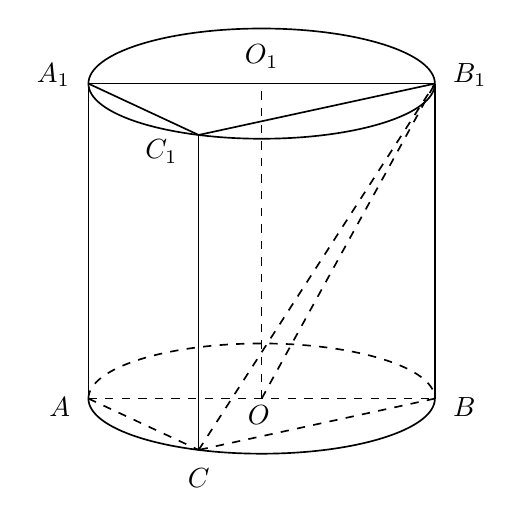
\begin{tikzpicture}[x=1cm,y=1cm,line width=0.6pt,font=\normalsize]
% cylinder approximated by two ellipses + sides
\coordinate (O) at (0,0);
\coordinate (O1) at (0,4);
\coordinate (A) at (-2.2,0);
\coordinate (B) at (2.2,0);
\coordinate (C) at (-0.8000000000,-0.6520786851);
\coordinate (A1) at (-2.2,4);
\coordinate (B1) at (2.2,4);
\coordinate (C1) at (-0.8000000000,3.3479213149);
% bottom ellipse: front solid, back dashed
\draw[solid] (-2.2,0) arc (180:360:2.2 and 0.7);
\draw[dashed] (-2.2,0) arc (180:0:2.2 and 0.7);
% top ellipse full
\draw[solid] (0,4) ellipse (2.2 and 0.7);
% sides
\draw[solid] (A)--(A1);
\draw[solid] (B)--(B1);
% axis
\draw[dashed] (O)--(O1);
% prism vertical
\draw[solid] (C)--(C1);
% top triangle
\draw[solid] (A1)--(B1);
\draw[solid] (A1)--(C1);
\draw[solid] (C1)--(B1);
% bottom triangle (hidden dashed)
\draw[dashed] (A)--(B);
\draw[dashed] (A)--(C);
\draw[dashed] (B)--(C);
% space diagonals to B1 (A-B diameter passes through O; O-B1 kinks there)
\draw[dashed] (C)--(B1);
\draw[dashed] (O)--(B1);
% labels with clearance
\node[left,xshift=-3pt,yshift=-3pt] at (A) {$A$};
\node[right,xshift=3pt,yshift=-3pt] at (B) {$B$};
\node[below,yshift=-3pt] at (C) {$C$};
\node[left,xshift=-3pt,yshift=3pt] at (A1) {$A_{1}$};
\node[right,xshift=3pt,yshift=3pt] at (B1) {$B_{1}$};
\node[left,xshift=-4pt,yshift=-6pt] at (C1) {$C_{1}$};
\node[below=2pt,xshift=-1pt,yshift=3pt] at (O) {$O$};
\node[above=2pt] at (O1) {$O_{1}$};
\end{tikzpicture}
